\documentclass{article}
\usepackage{blindtext}
\usepackage[utf8]{inputenc}
\usepackage{multicol,caption}
\usepackage[margin=1.0in]{geometry}
\usepackage{multirow}
\usepackage{array}
\usepackage{graphicx}
\newcommand\tab[1][1cm]{\hspace*{#1}} 
\newenvironment{Figure}
  {\par\medskip\noindent\minipage{\linewidth}}
  {\endminipage\par\medskip}
 
\title{\underline{Distributed Neural Networks} \\ \large Developed with JAMScript Architecture}
\author{  Prof. Muthucumaru Maheswaran - Brian Choi -  Alex Chung - Salman Memon \\ \normalsize McGill University School of Computer Science \\  \small \underline{maheswar@cs.mcgill.ca} - \underline{ga.choi@mail.mcgill.ca} - \underline{alex.chung@mail.mcgill.ca} - \underline{salman.memon@mail.mcgill.ca}  }
\date{\today}

\begin{document}

\maketitle

\section{Introduction}

\begin{multicols}{2}
The advent of cloud computing and efficient data transfer has allowed for machines with limited processing power and disk space to accomplish tasks previously impossible. Such highly connected networks of smaller CPUs is commonly referred to as an Internet of Things. Devices such as smart fridges, watches, cameras and cars make up this Internet of Things. JAMScript allows for efficient, limitless data transfer from the greater internet - the “cloud” - to the more restricted local area network, which we will henceforth refer to as the “fog”. The fog then communicates directly with devices on the local area network and facilitates process tasking and data sharing. The purpose of this project was to explore whether cutting edge machine learning algorithms and structures could be distributed across a network to allow even the most computationally restricted machines to recognize complex patterns.

\end{multicols}

\section{Machine Learning Overview}

\begin{multicols}{2}

	Machine learning is often divided into supervised, unsupervised, and reinforced learning. For this project, we focused on supervised learning due to availability of resources and it’s tendency to produce accurate results. Supervised learning can be further categorized into regression and categorization problems. Regression problems output continuous values. Predicted \% rise in a stock and evaluating the probability of a disease in a patient are common examples of regression problems. Categorization problems group inputs into a discrete set of outputs. A common categorization problem is character recognition - outputs are limited to a set of known characters. We chose to solve a categorization problem.
\par
There are a number of algorithms for solving categorization learning problems: feed forward neural networks perform well. In feed forward neural networks, the input problem (e.g. a picture of a character), has features extracted and represented as numerical values to be passed into the network. Features for a character recognition problem may be the pixels of the image; for a stock prediction problem a feature may be price last month. Each feature is a node in the input layer. In Figure 1, there are 2 features for the input problem. The numerical value of the feature is passed to every node in the next layer. The nodes in the output layer correspond to the possible categories of our problem: the network in Figure 1 solves a problem with 2 possible outputs. After the network has been computed, the nodes in the output layer take values bounded between 0 and 1: the probability that the input problem falls into that category.
\begin{Figure}
 \centering
 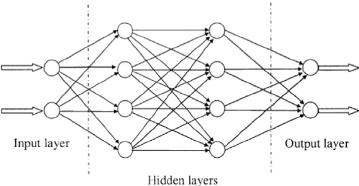
\includegraphics[width=\linewidth]{FFNN_Schematic}
 \captionof{figure}{A feed forward neural network schematic.}
\end{Figure}
	Layers between the input layer and the output layer are termed hidden layers. The majority of a neural networks computation occurs in these hidden layers. Each edge is associated with a numerical weight. Using Figure 1 as a visualization, each node in the first hidden layer takes as input the value of a node in the previous layer multiplied by its respective weight on the shared edge. Let nodes be denoted \(n_{i,j}\) where\( i\) denotes the layer number, 0-indexed starting from the input layer, and \(j\) denotes the node number within that layer. Let edges be denoted \(e_{i,j,k}\) where \(i\) denotes the layer number of the source, \(j\) denotes the node number of layer \(i\) that the edge starts from, and \(k\) denotes the node number in layer \(i+1\) that the edge ends on. Then the value inputted to \(n_{i+1,k}\) is \[\sum_{j}(n_{i,j}*e_{i,j,k}) + b_{i+1,k}\]
\(b_{i+1,k}\) denotes the bias of node \(n_{i+1,k}\). The significance of the bias \(b\) will be discussed in following paragraphs. Node \(n_{i+1,k}\)'s value is the result of calculating the sigmoid function: \[ S(x) = \frac{1}{1+e^{-x}} \] where x is the node's input. The sigmoid is a smooth function bounded by 0 and 1. After expansion \[S(x) = \frac{1}{1+e^{-\sum_{j}(n_{i,j}*e_{i,j,k}) + b_{i+1,k}}}\]. 
\par
	Intuitively, we can consider each node as a decision on some aspect of the problem: the input from all the previous layers, multiplied by the importance of their input (the edge weight) allows each node to determine if the feature exists (output a 1) or not (output a 0). As we progress further into the network, decisions become increasingly more abstract and based on decisions that have already occurred. Notice as \(b\), the bias increases, \(e^{-x}\) tends towards 0 and \(S(x)\) tends to 1. Therefore, we can describe a neuron’s bias as it’s tendency to consider some feature of the input problem as present regardless of inputs from the previous layer. The output of the sigmoid function is passed to nodes in the next layer. By using the sigmoid, a neural network gains more flexibility and can determine the probability that some aspect exists.
\par
	Utilizing the smooth nature of the sigmoid function allows for training of a neural network. When using a feed forward neural network, a large amount of data is required. Typically, a good data set will have upwards of 50 000 sample problems with their correct outputs. We split the data into a training and a testing set. First we randomly allocate edge weights. Then we test every problem in our training set and alter the value of the weight based on a correct or incorrect output.  We define a cost function that approaches 0 when output is correct and diverges from 0 as output is more incorrect. The more an output differs from the correct output, the more error our network has. As output is a function of all the weights and biases in a network, we can find the derivative of any weight or bias in the network and determine its contribution to the error. Using the gradient of the cost function, we can slowly alter the weights until our neural network has a high probability for correctness. After training is done, we test out network on a set of problems the network hasn’t seen yet - the test set. We iteratively keep training until the \% improvement on correct output falls below some small threshold \(\epsilon\). 

\end{multicols}

\section{JAMScript Overview}

\begin{multicols}{2}

JAMScript is an in-development polyglot language designed to address connection stability and latency issues for mobile device cloud systems. A cloud-fog-device architecture is proposed to help combat the aforementioned issues. JAMScript runs on Javascript and C.
Javascript portions of JAMScript programs execute networking tasks while C portions exist only on devices and address memory and CPU management. Javascript programs will be referred to as J-Nodes for the remainder of the paper and C programs will be referred to as C-Nodes Figure 2 demonstrates placement of J and C nodes within the structure. 
\begin{Figure}
 \centering
 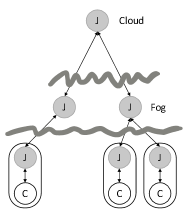
\includegraphics[width=4cm]{JAMScript_NN_Architecture}
 \captionof{figure}{Cloud-fog-device architecture.}
\end{Figure}
\newpage
The cloud facilitates data transfer using a J-Node. The fog then accesses that information using its own J-Node. A device, by joining a fog, can then utilize the data the fog has by reading information through the device's J-Node. Data processing in devices occurs through the C-Node, after communication with the J-Node. Top-down communication (from cloud to fog, fog to device, or device J to device C) can be facilitated with a number of different data stream types but our project utilized a broadcaster.  Unlike the HTTP protocol, data is not sent to a specific device or fog but broadcasted to all connections. J-Nodes in the cloud-fog-device architecture can then access all or a subset of the broadcasted values from higher layers.  In C-Nodes, programs operate on the last broadcasted value. Consequently, well designed JAMScript programs can avoid disconnection faults by allowing any connected system to perform operations on data without relying on a specific device. Our specific use of the broadcaster will be discussed later in this paper. 
\par
Bottom-up communication is implemented through a stream called a logger. Loggers, unlike broadcasters, subscribe to a value and call a function when that value is updated. Loggers, then, are similar to event emitters and listeners. The logger tracks declared variables by placing values in name separated, strongly typed, Queue-like structures.  As logger values are changed in a C or J-Node, callback functions are executed in higher levels of the network architecture.

\end{multicols}

\section{Target Design}

\begin{multicols}{2}
	Neural network structure is heuristically chosen by the developer. For each problem, weights between neurons in a feed forward neural network change based on the structure: networks may differ in the number of hidden layers and the number of nodes per layer. Different structures reap different benefits. The greater number of nodes in a layer, the greater the accuracy of a network; dividing neurons into multiple hidden layers generally increases speed of computation. Therefore, for each unique structure of a network per problem, weights and biases must be trained to perform optimally. 
\par
	The high storage capability of the cloud suggested to us that after training, the network’s weight and bias structure should be stored in a database in the cloud. Because our networks have a variable number of devices per fog, it is desirable to have multiple different structures. For fogs with more devices, computation is faster so we use a network with more neurons. However, for fogs with less devices, we may be willing to sacrifice accuracy for speed. Thus we may train multiple structures of networks and grant them a unique structure id. We save each structure id in a list referenced by a unique problem id in our cloud database. Available network structures are accessed by querying the database for the previously found problem id. The structure id maps to a list of ids for each layer of the network. Finally, all neuron information - id, weights, and bias - are stored as a list of objects that can be found by querying the database for the layer id previously found. 
\par 
As a result, we can save the multiple network structure solutions to a multitude of problems and access them when required. Devices maintain a list of the unique id’s corresponding to saved problems in our cloud database. When a device requires the solution to a problem that the cloud database has trained, it makes a request to the fog. The fog checks if the device’s problem has a corresponding neural network saved in the fog’s own database. If not, the fog makes a request to the cloud to receive the desired neural network. Networks can be replaced in the fog database with a least recently used (lru) strategy or other common methods. 
\par
	The fog then acts as a controller. All devices in the fog are sent the input and corresponding problem id. Neuron id, weights, bias and problem id are then stored as an object in a queue that is accessed by devices in the fog. When a device starts computation, the neuron is declared as under computation so that other devices do not begin calculation needlessly. If a device disconnects or faults, the fog assumes the neuron computation cannot finish and releases it so that some other device may act on it. As neuron values are computed they are returned to the fog. Once all neurons in a layer have completed, the fog sends their results  as input to the next layer. The fog enqueues the next layer’s neurons and the process recurses until the final output has been sent back to the requesting device.
\par
As fogs are LAN connected, latency for the fog to device connection is low. Furthermore, controlling tasking and weight storage in the fog allows the system to disconnect from the greater internet but maintain functionality. Refer back to Figure 1 and notice that when the number of neurons in the previous layer is large, the computation of the inputted dot product becomes expensive. Our design specifications provide for improved time cost and allow for neural networks to be utilized by underpowered CPUs. Our project sees the greatest time benefits on networks with a single, large hidden layer and is the least beneficial to small networks with a minimal amount of neurons. By associating a problem id to inputs, weights and biases, different problems can be computed simultaneously.

\end{multicols}

\section{Implementation Details}
\begin{multicols}{2}
A network of small, autonomous drones is a suitable sample problem for both JAMScript and a distributed neural network project. As such, our team chose a dataset that, when learned, evaluates a number of ultrasound readings and classifies how a robot should move into 5 categories: forward, slight and sharp right turns, and slight and sharp left turns \footnote{available through the UCI Machine Learning Repository: https://archive.ics.uci.edu/ml/datasets/Wall-Following+Robot+Navigation+Data}. The dataset can be trained when the robot utilizes 2, 4 or 24 sensors. Each sensor represents a feature input into the neural network. Typically, as the number of features increases, the problem more accurately resembles the real world state. Our results for a number of problem and network formats is displayed below. We vary input feature, hidden layer, and neuron quantities.
\end{multicols}
	\begin{center}
	\begin{tabular}{ |c|c c c c c| } 
	\hline
	Network ID & \# of inputs & \# of hidden layers & \# of neurons/layer & \% accuracy & Epochs \\ 
	\hline
	1 & 2 & 1 & 2 & 97.87 & 1000 \\ 
	2 & 2 & 1 & 4 & 98.9 & 1000\\ 
	3 & 4 & 1 & 4 & 98.75 & 1000\\ 
	4 & 4 & 2 & 4 & 99.27 & 2000\\
	5 & 24 & 1 & 10 & 92.59 & 1000\\  
	\hline
	\multicolumn{6}{c}{\small Training results for different network structures}
	\end{tabular}
	\end{center}
\begin{multicols}{2} 
	Due to the JAMScript fog implementation being in progress at the time of this project’s commencement, we simulated our distributed neural network design on one machine. We used a J-Node as the fog, and multiple C-Nodes as devices. Referring to JAMScript docs, the fog and cloud are typically only composed of a J-Node, while the device communicates with the fog through it’s J-Node and processes the obtained data in the C-Node. Thus, our implementation accurately replicates JAMScript’s intended architecture. 
\par
First, the fog assigns each device a unique id. Starting from the input layer, the fog sends an ordered float array of values and the associated problem id to all devices. Along with the input, to the fog controller also broadcasts a particular neuron’s unique weights, bias and integer id. The object broadcasted in our proof of concept, as well as the JAMScript broadcaster syntax is shown in figure 3.
\begin{Figure}
 \centering
 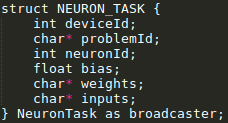
\includegraphics[width=5cm]{neuron_task}
 \captionof{figure}{Broadcasted neuron object.}
\end{Figure}
Each device performs the necessary dot product and calculations for neurons that have been assigned to it and returns the output, problem id, and neuron id to the fog. It is paramount that neurons are assigned unique ids because the value they pass to the following layer is multiplied by the weight on each edge from that specific neuron.
\begin{Figure}
 \centering
 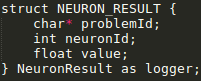
\includegraphics[width=4.5cm]{neuron_result}
 \captionof{figure}{Logged neuron result.}
\end{Figure}
The fog accumulates the output returned by devices in a float array. When the fog has received all the computed outputs, it broadcasts the output array as the new input to the corresponding problem’s next layer. This process happens iteratively until the network is complete and the output is returned to the requesting device. The fog continues to assign neurons, looping through the available devices until all  neurons in a layer are assigned. 
\end{multicols}
\newpage
\section{Extensions}
\begin{multicols}{2}
	Due to the high iteration count, training of neural networks is computationally expensive. The cloud presents a powerful solution for training networks and storing weights and biases. We decided the best demonstration of JAMScript’s capabilities and intended use would lie within the application rather than training of a distributed neural network. JAMScript is intended for use by an Internet of Things that require quick and accurate answers to problems. Naively implementing a distributed training scheme would over burden such networks. Futher, due to time constraints and the high difficulty of implementing the back propogation training algorithm, we decided to train and extract the weights and biases of a network using the powerful Keras python framework. A possible and impactful extension to this project would be to determine whether distributing training algorithms could be done efficiently with significant time benefits. 
\par
	Mutual exclusion on networked resources is a common problem with many effective solutions. For our target design to be implemented, mutual exclusion should be researched from a JAMScript perspective. A queue of neurons is more flexible and fault-tolerant than the assignment scheme.
\end{multicols}

\begin {center}
Special thanks to Lilly Jiang for her help with JAMScript - lilly.jiang@mail.mcgill.ca
\end{center}

\section{Resources}
\begin{itemize}
	\item Michael A. Nielsen - "Neural Networks and Deep Learning", Determination Press, 2015
	\item ANRL JAMScript - https://github.com/anrl/JAMScript-beta
	\item Python Keras - https://keras.io
\end{itemize}
\end{document}